\documentclass[10pt]{article}
\usepackage{amsmath, amssymb}
  \usepackage{graphicx}
  \usepackage{physics}
  \usepackage{siunitx}
  \usepackage[version=4]{mhchem}
  %\usepackage[utf8x]{inputenc}
  \usepackage{pifont}
  \usepackage{xcolor}
  \usepackage{listings}
  \usepackage{wasysym}
  \usepackage{tikz}
  \usepackage[clock]{ifsym}
  \usepackage{fontspec}
  \usepackage[compat=1.0.0]{tikz-feynman}
  \usepackage{chemfig}
  \usepackage{verbatim}
  \usepackage{skak}
  \usepackage{phaistos}
  \usepackage{pgfplots}
  \usepackage{pgf-pie}
  \usepackage{mathtools}
  \usetikzlibrary{arrows}
  \usetikzlibrary{snakes}
  \usepackage{chessfss}



  \usepackage{etoolbox}
  \newtoggle{showpct}
  \makeatletter
  \patchcmd{\pgfpie@slice}%
  {\scalefont{#3}\beforenumber#3\afternumber}%
  {\iftoggle{showpct}{\scalefont{#3}\beforenumber#3\afternumber}{}}%
  {}{}
  \makeatother

  \usepackage{polyglossia}
  \setdefaultlanguage{english}
  \setotherlanguage{korean}

  \defaultfontfeatures{Scale = MatchUppercase}
  \newfontfamily\koreanfont{Noto Serif CJK KR}[Script = Hangul, Language = Korean]
  \newfontfamily\koreanfontsf{Noto Sans CJK KR}[Script = Hangul, Language = Korean]


  \tikzset{
    treenode/.style = {align=center, inner sep=0pt, text centered,
      font=\sffamily},
    arn_n/.style = {treenode, circle, black, draw=black,
      fill=white, text width=1.5em},% arbre rouge noir, noeud noir
  }


  \def\slant#1#2{%
    \tikz[baseline=(X.base), xslant=tan(#1)]
      \node[inner sep=0pt, xslant=tan(#1)](X){#2};%
  }

  \makeatletter
  \newsavebox\myboxA
  \newsavebox\myboxB
  \newlength\mylenA

  \newcommand*\xoverline[2][0.75]{%
      \sbox{\myboxA}{$\m@th#2$}%
      \setbox\myboxB\null% Phantom box
      \ht\myboxB=\ht\myboxA%
      \dp\myboxB=\dp\myboxA%
      \wd\myboxB=#1\wd\myboxA% Scale phantom
      \sbox\myboxB{$\m@th\overline{\copy\myboxB}$}%  Overlined phantom
      \setlength\mylenA{\the\wd\myboxA}%   calc width diff
      \addtolength\mylenA{-\the\wd\myboxB}%
      \ifdim\wd\myboxB<\wd\myboxA%
         \rlap{\hskip 0.5\mylenA\usebox\myboxB}{\usebox\myboxA}%
      \else
          \hskip -0.5\mylenA\rlap{\usebox\myboxA}{\hskip 0.5\mylenA\usebox\myboxB}%
      \fi}


  \newcommand\strictCeil[1]{\left|\!\xoverline[1.1]{#1}\!\right|}

  \newcommand\superS[1]{
    \begin{tikzpicture}[y=0.80pt, x=0.80pt,inner sep=0pt, outer sep=0pt, baseline=-0.95em, rotate=180, transform shape, scale=#1]
  \begin{scope}[cm={{0.1,0.0,0.0,-0.1, (25.51618,413.50385)}},fill=black,xscale=-1]
    \path[fill] (638.2500,3351.0000) .. controls (140.2500,2748.0000) and
      (0.0000,2574.7500) .. (1.5000,2563.5000) .. controls (4.5000,2544.0000) and
      (2257.5000,-1.5000) .. (2268.7500,1.5000) .. controls (2286.0000,5.2500) and
      (4500.0000,2553.0000) .. (4497.7500,2566.5000) .. controls
      (4497.0000,2573.2500) and (4316.2500,2775.0000) .. (4096.5000,3014.2500) --
      (3696.0000,3450.0000) -- (2208.0000,3450.0000) -- (720.0000,3450.0000) --
      cycle(3283.5000,3163.5000) .. controls (3265.5000,3141.7500) and
      (3227.2500,3095.2500) .. (3198.7500,3060.7500) -- (3147.0000,2998.5000) --
      (3132.0000,3019.5000) .. controls (3124.5000,3031.5000) and
      (3081.7500,3077.2500) .. (3037.5000,3122.2500) -- (2958.0000,3202.5000) --
      (3137.2500,3202.5000) -- (3316.5000,3202.5000) -- cycle(1066.5000,3158.2500)
      .. controls (825.7500,3014.2500) and (671.2500,2833.5000) ..
      (615.7500,2632.5000) .. controls (591.0000,2544.7500) and (582.0000,2437.5000)
      .. (591.0000,2351.2500) .. controls (595.5000,2310.7500) and
      (598.5000,2276.2500) .. (597.7500,2274.7500) .. controls (594.0000,2271.7500)
      and (288.7500,2616.7500) .. (288.7500,2624.2500) .. controls
      (288.7500,2628.0000) and (396.7500,2758.5000) .. (528.7500,2913.0000) --
      (768.7500,3194.2500) -- (948.0000,3194.2500) -- (1127.2500,3195.0000) --
      cycle(2366.2500,3176.2500) .. controls (2504.2500,3153.7500) and
      (2628.7500,3106.5000) .. (2728.5000,3038.2500) .. controls
      (2851.5000,2955.0000) and (2961.7500,2799.0000) .. (3012.0000,2638.5000) --
      (3025.5000,2595.0000) -- (3402.7500,2595.0000) -- (3780.0000,2595.0000) --
      (3781.5000,2811.7500) -- (3783.7500,3029.2500) -- (3987.0000,2798.2500) --
      (4191.0000,2567.2500) -- (3934.5000,2311.5000) -- (3678.7500,2056.5000) --
      (3615.0000,2122.5000) .. controls (3435.7500,2307.7500) and
      (3218.2500,2403.7500) .. (2883.7500,2446.5000) .. controls
      (2832.0000,2452.5000) and (2679.0000,2456.2500) .. (2392.5000,2456.2500) ..
      controls (1950.0000,2457.0000) and (1950.0000,2457.0000) ..
      (1795.5000,2496.7500) .. controls (1571.2500,2553.7500) and
      (1378.5000,2680.5000) .. (1338.7500,2796.7500) .. controls
      (1314.0000,2870.2500) and (1328.2500,2919.0000) .. (1395.0000,2985.7500) ..
      controls (1502.2500,3093.7500) and (1719.0000,3162.7500) ..
      (2032.5000,3190.5000) .. controls (2097.0000,3196.5000) and
      (2298.7500,3187.5000) .. (2366.2500,3176.2500) -- cycle(1346.2500,1830.0000)
      .. controls (2328.0000,1782.0000) and (2822.2500,1713.7500) ..
      (3047.2500,1595.2500) .. controls (3096.7500,1569.7500) and
      (3142.5000,1522.5000) .. (3142.5000,1498.5000) .. controls
      (3142.5000,1470.0000) and (3069.0000,1407.0000) .. (2991.0000,1369.5000) ..
      controls (2857.5000,1305.0000) and (2696.2500,1268.2500) ..
      (2516.2500,1262.2500) .. controls (2346.7500,1256.2500) and
      (2237.2500,1277.2500) .. (2180.2500,1326.0000) .. controls
      (2076.0000,1416.7500) and (1910.2500,1478.2500) .. (1710.0000,1500.7500) ..
      controls (1579.5000,1515.0000) and (1416.0000,1497.0000) ..
      (1343.2500,1459.5000) -- (1320.7500,1447.5000) -- (1165.5000,1633.5000) ..
      controls (1080.0000,1735.5000) and (1005.0000,1824.7500) ..
      (999.0000,1832.2500) .. controls (984.7500,1848.7500) and (962.2500,1848.7500)
      .. (1346.2500,1830.0000) -- cycle(2751.7500,945.0000) .. controls
      (2725.5000,908.2500) and (2275.5000,375.7500) .. (2271.7500,377.2500) ..
      controls (2265.0000,379.5000) and (1770.0000,947.2500) .. (1772.2500,949.5000)
      .. controls (1773.7500,951.0000) and (1800.7500,943.5000) ..
      (1833.0000,933.7500) .. controls (2030.2500,873.0000) and (2257.5000,857.2500)
      .. (2471.2500,888.7500) .. controls (2545.5000,900.0000) and
      (2668.5000,929.2500) .. (2718.7500,948.0000) .. controls (2759.2500,963.0000)
      and (2763.7500,962.2500) .. (2751.7500,945.0000) -- cycle;
  \end{scope}
  \end{tikzpicture}
  }
  \definecolor{rot}{HTML}{E40303}
  \definecolor{xorange}{HTML}{FF8C00}
  \definecolor{gelb}{HTML}{FFED00}
  \definecolor{gruen}{HTML}{008026}
  \definecolor{blau}{HTML}{004DFF}
  \definecolor{lilla}{HTML}{750787}

  \newcommand\pride[1]{  \begin{tikzpicture}[scale=#1,inner sep=0pt, outer sep=0pt,transform shape, baseline=-0.95em]
    \begin{scope}
      \foreach[count=\i] \col in {lilla,blau,gruen,gelb,xorange,rot}
        \fill[\col] (0,7*\i) rectangle +(75,7);
    \end{scope}
    \end{tikzpicture}}
    
    
  \newcommand{\prideflag}{\pride{0.005}}

  \newcommand{\Superman}{\superS{0.03}}

  \def\molecule#1#2#3#4#5#6#7{
  \begin{scope}[shift=#1,rotate=#2]
      \draw [fill=black] (0,0) circle (.5);
      \draw (0,-0.5) -- (0,-0.5-#3);
      \draw (0,-0.8-#3) circle (.3);
      \draw ({0.5*cos(#6)},{-0.5*sin(#6)}) -- ({(0.5+#4)*cos(#6)},{-(0.5+#4)*sin(#6)});
      \draw ({(0.8+#4)*cos(#6)},{-(0.8+#4)*sin(#6)}) circle (.3);
      \draw ({0.5*cos(#7)},{0.5*sin(#7)}) --({(0.5+#4)*cos(#6)},{-(0.5+#4)*sin(#6)});
  \end{scope}
  }


  \newcommand{\orcapre}[1]{
  \begin{tikzpicture}[y=0.80pt, x=0.80pt, yscale=-#1, xscale=#1, inner sep=0pt, outer sep=0pt,baseline=-0.7em]
   \path[draw=black,fill=black,line width=0] (506.5380,198.4650) ..
      controls (503.4870,204.2380) and (491.5530,219.9830) .. (481.7170,224.3210) ..
      controls (462.6960,231.6900) and (456.1720,231.3240) .. (450.6890,229.4930) ..
      controls (447.0610,228.9630) and (449.6490,222.6210) .. (450.6890,220.1840) ..
      controls (450.9620,217.3690) and (462.7800,200.9550) .. (468.2720,195.3630) ..
      controls (474.6010,190.4480) and (506.5380,198.4650) .. (506.5380,198.4650) --
      (506.5380,198.4650) -- cycle;



    \path[draw=black,fill=black,line width=0] (109.3840,193.2970) ..
      controls (109.3840,193.2970) and (92.4680,218.6820) .. (74.2180,221.2200) ..
      controls (55.7010,223.9340) and (33.3770,217.3690) .. (25.6090,221.2200) ..
      controls (17.6190,225.2470) and (9.7410,227.8730) .. (5.9580,233.6300) ..
      controls (12.3650,234.4390) and (14.9940,227.8730) .. (19.4040,234.6650) ..
      controls (22.8740,241.0080) and (29.4390,244.9460) .. (36.9870,246.0410) ..
      controls (45.1970,247.5680) and (37.3150,251.5120) .. (42.1570,253.2830) ..
      controls (47.8240,254.1370) and (62.2650,255.4500) .. (64.9120,268.7960) ..
      controls (67.5190,281.7160) and (68.0140,281.2060) .. (68.0140,281.2060) ..
      controls (68.0140,281.2060) and (63.5810,300.0980) .. (55.6030,303.9610) ..
      controls (62.2650,305.3500) and (92.4690,307.9760) .. (98.0070,280.1750) ..
      controls (102.9750,252.8250) and (88.5290,244.9460) .. (102.1440,236.7360) ..
      controls (114.7920,229.1870) and (177.1800,204.2150) .. (211.7770,195.3640) ..
      controls (230.4000,190.0780) and (257.7580,185.8060) .. (291.4150,186.0540) ..
      controls (333.8250,187.3710) and (383.3370,204.2050) .. (436.2120,199.5000) ..
      controls (479.5590,194.7530) and (613.1330,202.9260) .. (599.6240,192.2620) ..
      controls (613.1330,184.5390) and (603.5040,157.4200) .. (585.1430,136.4120) ..
      controls (567.8300,116.2580) and (457.5270,88.6800) .. (441.3840,84.6990) ..
      controls (435.2740,83.1160) and (410.2540,23.0200) .. (386.5650,7.1290) ..
      controls (386.5650,7.1290) and (365.6080,0.6990) .. (381.3930,29.8840) ..
      controls (386.6160,32.2160) and (413.6250,85.0350) .. (353.4700,83.6630) ..
      controls (284.9210,82.4900) and (169.2950,92.4680) .. (109.3840,193.2970) --
      (109.3840,193.2970) -- cycle;



    \path[draw=black,fill=white,line width=0]
      (336.9220,191.2260) .. controls (260.6450,180.0200) and (205.5690,196.3990) ..
      (205.5690,196.3990) .. controls (210.3750,190.4950) and (290.5840,153.8810) ..
      (367.9510,152.9600) .. controls (403.2050,151.8540) and (381.7420,198.4200) ..
      (377.2560,197.4350) .. controls (363.6540,195.4680) and (349.6830,192.9820) ..
      (336.9220,191.2260) -- (336.9220,191.2260) -- cycle;



    \path[fill=white,line width=0] (501.3700,151.9240) .. controls (527.7490,133.9290) and
      (562.0980,137.0090) .. (560.3220,150.8930) .. controls (559.2950,162.2180) and
      (541.2240,164.8440) .. (531.3630,164.3350) .. controls (519.9040,164.8440) and
      (477.8790,168.1260) .. (501.3700,151.9240) -- (501.3700,151.9240) -- cycle;



    \path[draw=black,fill=white,line width=0]
      (426.9020,199.5000) .. controls (444.7750,187.7630) and (443.4750,164.8440) ..
      (504.4710,173.6440) .. controls (516.8730,175.1040) and (624.6010,191.0290) ..
      (594.4510,196.3990) .. controls (552.7290,203.5790) and (551.1550,201.6130) ..
      (493.0960,202.6060) -- (426.9020,199.5000) -- (426.9020,199.5000) -- cycle;



    \path[draw=black,fill=black,line width=0] (491.0260,161.2340) ..
      controls (487.7300,164.8440) and (466.7180,171.4100) .. (457.9310,171.5780) ..
      controls (448.3350,171.4100) and (397.7760,192.4220) .. (388.6350,204.6730) ..
      controls (379.3930,217.3700) and (382.6750,221.9650) .. (384.4970,225.3580) ..
      controls (386.6140,228.5310) and (439.1400,220.0010) .. (450.6870,211.9120) ..
      controls (461.4650,204.2400) and (482.4730,193.7360) .. (486.8870,188.1260) ..
      controls (491.6640,181.9190) and (498.2630,173.6460) .. (498.2630,173.6460);

  \end{tikzpicture}
  }

  \newcommand{\orca}{\orcapre{0.03}}

  \def\rotatechartwo#1{\reflectbox{#1}}

  \definecolor{hanpurple}{rgb}{0.32, 0.09, 0.98}
  %\newcommand{\knightB}[1][1.85ex]{%
  %\adjustbox{Trim=3.2pt 2.2pt 3.2pt 0pt, width=#1, raise =-0.03ex,margin=0.14ex 0ex 0.14ex 0ex}{\BlackKnightOnWhite}%
  %}
  \def\x2o#1#2#3{
  \begin{scope}[shift={#1},rotate=#2, inner sep=0pt]
    \draw  (0.6,0) node[circle,fill=white] {#3} -- (0,0) node[circle, fill=white] {O} -- ({+0.6*cos(104.5)},{0.6*sin(104.5)}) node[circle, fill=white] {#3};
  \end{scope}
  }




  \begin{document}
  1 Film [2]
  \[\begin{split}
  \left \lceil{\phantom{x}} \right \rceil& \\
  e&  \\
  \left \lfloor{\phantom{x}}\right \rfloor & \\
  \end{split}
  \]

  2 Film [2]
    \[
      -\log_{10}(\text{InnateBehaviour}) > 7
    \]

  3 Song [3]
  \[
  \heartsuit = \frac{1}{c^2}\pdv[2]{}{t} - \pdv[2]{}{x} - \pdv[2]{}{y} - \pdv[2]{}{z} 
  \]

  4 Film [1]
  \[
  \lim_{x \to a} f(x) \text{ undefined}
  \]

  5 Film/Book [3]
  \[
  p(x)= |\psi(x)|^2
  \]

  6 Song [2]
  \[
   \vec{E} = \vec{E}_0 e^{-t/\tau}
  \]

  7 Film [1]
  \[
    0\text{b}111
  \]

  8 Show [4]
  \[
     \frac{\tan x}{\sin x} + c_T
  \]

  9 Game [2]
  \[
    \tau \ln 2
  \]

  10 Game [2]
  \[
     \dot{A}_2
  \]

  11 Song [4]
  \[
  \text{2U} \not\equiv \text{everything else}
  \]

  12 Book/Film [2]
  \[
  \sum_{i = 1}^{N} P(\text{(VeryGood})_i)(\text{VeryGood})_i
  \]

  13 Film [2]
  \[
     \text{Si}(x) \cos(x) +   \text{Si}(x) \cos(x) +   \text{Si}(x) \cos(x) +   \text{Si}(x) \cos(x) +   \text{Si}(x) \cos(x) +   \text{Si}(x) \cos(x) +   \text{Si}(x) \cos(x) 
  \]

  14 Album [2]
  \[
    y = mx + c, y = mx + d, y = mx + e
  \]


  \newpage

  15 Show [3]
  \[
  \texttt{\$ ls *.x}
\]
  16 Film [4]
  \[
   )2=t(\to)1=t(
  \]

  17 Album/Song [2]
  \[
  \color{hanpurple}
  \text{H}_2\text{O}
  \]

  \color{black}
  18 Album (also an unrelated Song works) [3] [4]
  \[
  \sup \{ \heartsuit \}
  \]


  19 Book/Film [6]
  \[
    \phi(t) = \frac{2\pi  t }{80} 
  \]

  20 Book/Film [2]
  \[
  \SI{233}{ \celsius} = \SI{506}{\kelvin} = 
  \]

  21 Film [3]
  \[ 
  \begin{split}
  &ma = mg - \underbrace{F_1}_{\text{this}} - F_2 \\
  & F_1 = \gamma_1 v \\
  &F_2 = \gamma_2 v^2 \\
  \end{split}
  \]

  22 Book [2]
  \[
  \vec{g}, \text{ } (\vec{E}, \vec{B}), \text{ } \underbrace{(\text{\ding{65}},\text{Cu})}_{\text{this}}
  \]

  23 Song [2]
  \[\begin{split}
  F_{}/&A\\
  \downarrow&\\
  \text{you ar}&\text{e here} \\
  \end{split}
  \]
   
  24 Film [3]
   \[
   \ce{La3Nd}
   \]
   
  25  Film [1]
   \[
  \frac{GMm}{r^2}
   \]
   
   
   26 Song [2]
   \[
   P(\female_1 \cap \female_2) = P(\female_1)P(\female_2)
   \]
   
  27 Song [4]
   \[
   KE_{\text{Stone}} = \tfrac12 m v^2 + \tfrac12 I \omega^2
   \]
   
  28 Book/Film [2]
   \[
   \begin{split}
  & D: \text{ discharged}\\
  & M: \text{ mentally unsound} \\
  & E: \text{ evaluation requested} \\
  &1. \text{ }D \implies (M \land E) \text{ (premise 1)} \\
  &2. \text{ }M \implies \neg E \text{ (premise 2)} \\
  &3. \text{ From 2, } \neg M \lor \neg E \\
     &4. \text{ From 3, } \neg(M \land E) \\
  &5. \text{ From 1 and 4, } \neg D 
  \end{split}
  \]

\[
   \begin{split}
  & S: \text{ new office toner supplied}\\
  & T: \text{ ran out of office toner} \\
  & R: \text{ requisition form printed and filled in} \\
  &1. \text{ }S \implies (T \land R) \text{ (premise 1)} \\
  &2. \text{ }T \implies \neg R \text{ (premise 2)} \\
  &3. \text{ From 2, } \neg T \lor \neg R \\
  &4. \text{ From 3, } \neg(T \land R) \\
  &5. \text{ From 1 and 4, } \neg S
  \end{split}
  \]


  29 Film [4]
  \[
  e^{i\pi} + 1 = 0 \text{ and } 666
  \]

  30 Film [1]
  \[
    d(d(d(x)))
  \]

  31  Book/Film [3]
   \[\begin{split}
     &\int_{a}^{b}  \vec{F}_\text{\showclock{0}{45}} \cdot \dd{\vec{r}},\\
    &b-a = o\\
    \end{split}
   \]
   
   32 Film/Book [3] 
   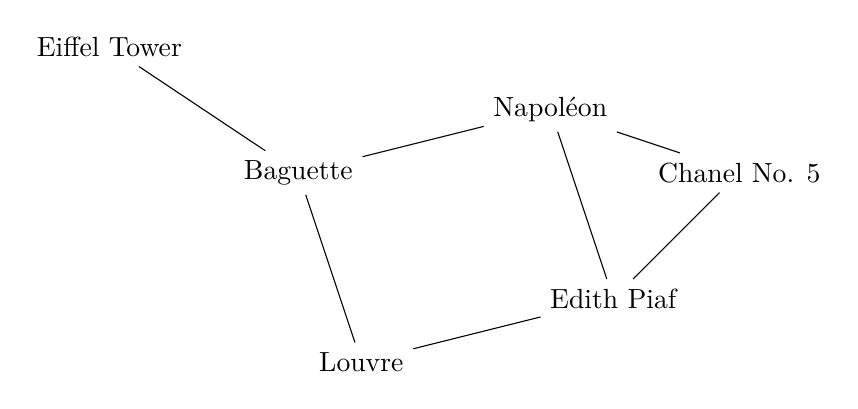
\begin{tikzpicture}
    [scale=.8,auto=left]
    \node (n6) at (1,10) {Eiffel Tower} ;
    \node (n4) at (4,8)  {Baguette};
    \node (n5) at (8,9)  {Napol\'eon};
    \node (n1) at (11,8) {Chanel No. 5};
    \node (n2) at (9,6)  {Edith Piaf};
    \node (n3) at (5,5)  {Louvre};

    \foreach \from/\to in {n6/n4,n4/n5,n5/n1,n1/n2,n2/n5,n2/n3,n3/n4}
      \draw (\from) -- (\to);

  \end{tikzpicture}
   
  33 Film/Book [2]
  \[
  \neg(\text{PhD})
  \]

  34 Song [3]
  \[
   \female \in \mathbb{N}
  \]

  35 Album/Song/Film [4]
  \[
  \forall \text{{\fontspec{FreeSerif}⚖}}
  \]

  36 Film [2]
  \[ 
  \text{Life}(t + \text{24hr}) = \text{Life}(t)
  \]

  37 Film [3]
  \[
  \text{Lost} \to \text{Lost} + \Delta x 
  \]

  38 Film [5]
  \[
  \text{Target: } \int \sqrt{1 + \left(\dv{\text{Missing}}{x}\right)^2} \dd{x}
  \]

  39 Film/Game [1]
  \[
  \frac{c}{d}\sqrt{-1} = \frac{c+d}{c}\sqrt{-1}
  \]

  40 Film [1]
  \[
  \pdv{u}{t} = \alpha \nabla^2 u
  \]

  41 Film [3]
  \[
    \begin{pmatrix}
  \cos \theta & -\sin \theta \\
  \sin \theta & \phantom{-}\cos \theta \\
  \end{pmatrix}
  \]

  42 Film [1]
  \[
  \tan \hat{\male}
  \]

  43 Film [4]
  \[
  \begin{split}
  \text{Python: }& (-3,4)\\
  \text{Anaconda: }& (1,-3)\\
  \text{Cobra: }& (4,5) \\
  \text{Viper: }& (-1,-2)\\
  \end{split}
  \]

  44 Film/Book [2]
  \[
  \sin(\text{London})
  \]

  45 Game [2]
  \[
  (d,17), (e,3), (i,13), (m,2), (o,11), (r,7)  , (t,5) 
  \]

  46 Song [2]
  \[
  \begin{split}
  &\text{If A is 1, B is 10, C is 11, etc} \\
   &\text{what is 1100 1111 10110 101?} \\
  \end{split}
  \]

  47 Song [1]
  \[
    \dv{W}{t}
  \]

  48 Song [4]
  \[
   ( u \in \phi ) \lor ( u \not\in \phi)
  \]

  49 Song [1]
  \[
    f: X \to Y, \text{ } g: X \to Y, \text{ } h: X \to Y
  \]

  50 Song [3]
  \[
    \sum_{i }^{\heartsuit} \text{\textkorean{웃}}_i 
  \]

  51 Show [1]
  \[
    t - 30 
  \]

  52 Book/Film [1]
  \[
    \$^2 + €^2 + £^2 \leq R^2
  \]

  53 Film [2]
  \[
    \text{False} \implies \text{False}
  \]

  54 Game [2]
  \[
    (\ce{D2O})_{\SI{\approx 0.003}{\mol}}
  \]
   
   \begin{figure}[htbp!]
     \begin{tikzpicture}
      \coordinate (a) at (0,1.5);% Change 1.5 to change the shape of the droplet
       \node [circle,draw,fill=white] (c) at (0,0) [minimum size=40pt] {};
    \fill[white] (a) -- (tangent cs:node=c,point={(a)},solution=1) --
    (c.center) -- (tangent cs:node=c,point={(a)},solution=2) -- cycle;
       \draw    (tangent cs:node=c,point={(a)},solution=1) -- (a) --
     (tangent cs:node=c,point={(a)},solution=2);
       \draw (0,0) -- ++(-40:2);
       \draw (-40:4) circle (2);
        \x2o{(2.5,-2)}{0}{D};
        \x2o{(1.8,-2.5)}{0}{D};
        \x2o{(3,-1.5)}{0}{D};
        \x2o{(3,-2.5)}{-100}{D};
        \x2o{(2.8,-3.5)}{-120}{D};
        \x2o{(4.1,-3.2)}{-100}{D};
        \x2o{(2,-3.2)}{150}{D};
        \x2o{(4.1,-2.1)}{-40}{D};
        







     \end{tikzpicture}
  \end{figure}

  \begin{figure}[htbp!]
    \begin{tikzpicture}
      
    \end{tikzpicture}
  \end{figure}


  55 Film [3]
  \[
  \feynmandiagram [horizontal=a to b] {
    i1 [particle =\(\text{Distressed}\)]  -- [fermion] a -- [fermion] b,
    i2 [particle =\(\text{Comfort}\)] -- [photon] a,
  };
  \]

  \begin{figure}[htbp!]
  \centering
    \begin{tikzpicture}
      \draw (0,0) --(2,0)  node[right] {Distressed};
      \draw (0,2) -- (2,2);
      \draw[->] (1,0) -- (1,2);
      
       \tikzset{decoration={snake,amplitude=.4mm,segment length=2mm,
                         post length=1mm,pre length=0mm}};
                         
          \draw[decorate,->] (2.5,1.5) node[right]{Comfort} -- (1.2,0);
          
          \draw[->] (-1,-1) -- (-1,3) node[above] {$E$}; 
    \end{tikzpicture}
  \end{figure}

  56 Film [2]
  \[
  \begin{tikzpicture}[domain=0:2, scale = 3]
   \draw (1.3,0) circle [radius = 0.2]; 
   \draw[->] (1.35,0.19364916731) arc (50: 220: 1.3 and 0.5);
   \draw (-0.5,-0.2) circle [radius = 0.2] node {$x$};
  \end{tikzpicture}
  \]

  57 Book [2]
  \[
    \text{Horse} \leq \text{Dog} \leq \text{Pig}
  \]

  58 Song [3]
  \[
    > m\text{word} 
  \]

  59 Film [2]
  \[
    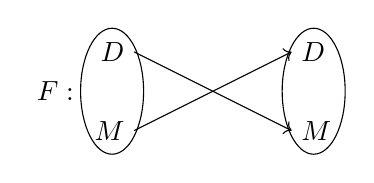
\begin{tikzpicture}
      \draw[->] (0,-0.5) node[left] {$M$} -- ( 2,0.5) node[right] {$D$};
      \draw[->] (0, 0.5) node[left] {$D$} -- (2,-0.5) node[right] {$M$};
      \node at (-1,0) {$F:$};
      \draw (-0.28,0) circle (0.4 and 0.8);
      \draw (2.28,0) circle (0.4 and 0.8);
    \end{tikzpicture}
  \]

	60 Film [3] and Film/Book [1]
  \[
    r_{\male_1}<\frac{2GM_1}{c^2}, \quad r_{\male_2} < \frac{2GM_2}{c^2}
  \]

  61 Show [2]
  \[
   \schemestart
    \chemfig{@{a2}{Ba} -[@{a1}]{\phantom{.}^2H}}
   \arrow{->} 
   \chemmove{\draw[->](a1).. controls +(90:6mm) and +(80:6mm).. (a2);}
    \chemfig{@{a3}{Ba^-}}
   \chemfig{\phantom{EE}}
    \chemfig{@{a4}{\phantom{.}^2H^+}}
   \schemestop
   \]
  62 Film [1]
  \begin{table}[htbp!]
    \begin{tabular}{c}
       Average bond energy(\si{\kilo\joule\per\mol})\\
         \infty  \\
    \end{tabular}
  \end{table}

  63) Song [4] 
  \[
    \ce{H2O} \text{ }\ce{O2}\text{ }  \text{\symknight} \text{ } \ce{N2} \text{ }\text{\symknight} \text{ }\ce{CO2}\text{ }  \ce{Ar} 
  \]

  64) Song [5] 
  \begin{figure}[htbp!]
  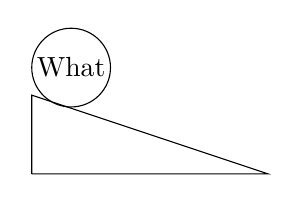
\begin{tikzpicture}
    \draw[-] (0,0) -- (3,0) -- (0,1) -- (0,0);
    \draw (0.5,0.85+0.5) circle (0.5) node {What}; 
  \end{tikzpicture}
  \end{figure}

  65) Song [2]
    \begin{figure}[htbp!]
      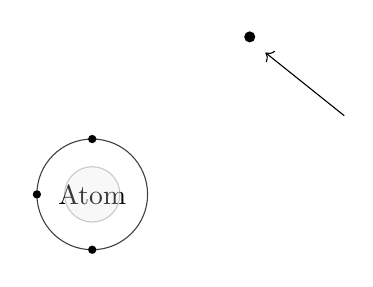
\begin{tikzpicture}[,
  baseline=(nucleus.base),
    nucleus options/.style = {draw=black!80,fill=black!10,opacity=.25},
    shell options/.style = {draw=black!75,thin},
    silicon/.pic = {
      \node(nucleus) at (0,0) {Atom};
      \draw[nucleus options] (nucleus) circle (1em);
      \draw[shell options] (nucleus) circle (2em);
      \foreach \angle in {90,180,270} {
        \fill (nucleus) ++(\angle:2em) circle (1.5pt) node {\PHeagle};
      }
    },
    scale=2
    ]
    \path (0,0) pic {silicon};
    \fill (1,1) circle (1pt) node {\PHeagle};
    \draw[->] (1.6,0.5) -- (1.1,0.9); 
  \end{tikzpicture}
  \end{figure}

  66) Album [9]
  \[
    \text{me} = \{ \lnot A| \text{Any proposition of the form: } A \in \text{me} \} 
  \]

  67) Album [2]
    \[
      \text{XOR}
    \]

  68) Album [4]
  \begin{figure}[htbp!]
    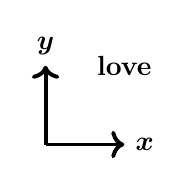
\begin{tikzpicture}
      \draw[line width = .5mm,->] (0,0) -- (0,1) node[above] {$\boldsymbol{y}$};
      \draw[line width = .5mm,->] (0,0) -- (1,0) node[right] {$\boldsymbol{x}$};
    \node at (1,1) {\textbf{love}};
    \end{tikzpicture}
    \end{figure}

  69) Album [2]
    \togglefalse{showpct}
    \begin{figure}[htbp!]
    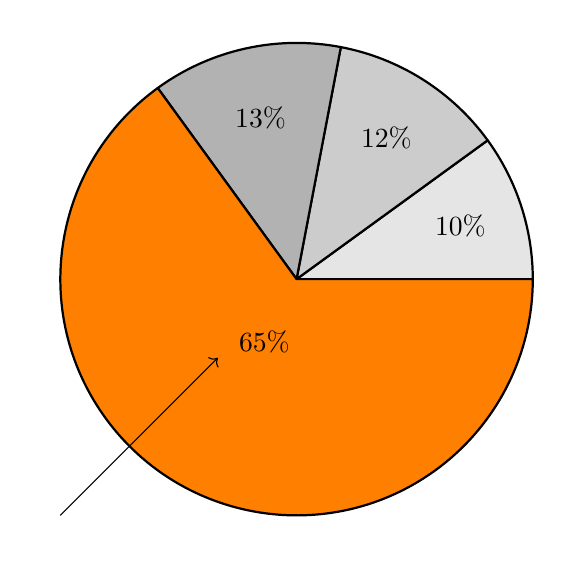
\begin{tikzpicture}
    \pie [
              color = {black!10, black!20, black!30, orange}] {   10/,  12/,  13/, 65/};
            \draw[->] (-3,-3) -- (-1,-1);
    \end{tikzpicture}
      \caption{Particle decay products}
    \end{figure}
    
    70) Song [2]
    \[
      \begin{split}
        &\text{The distance of X from Sun where} \\
        &\frac{\text{Distance of X from Sun}}{\text{Distance of Earth from Sun}} = \text{fools}\\
      \end{split}
      \]

    71) Album/Songs [4]
    \begin{figure}[htbp!]
      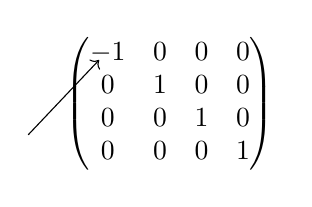
\begin{tikzpicture}
        \draw[->] (-1.3,0.1) -- (-0.4,1.05);
        \node at (0.5,0.5) {$\begin{pmatrix}
        -1 & 0 & 0 & 0 \\
        0 & 1 & 0 & 0 \\
        0 & 0 & 1 & 0 \\
        0 & 0 & 0 & 1 \\
        \end{pmatrix}$};
      \end{tikzpicture}
    \end{figure}

    72) Film [1]
    \[
      \texttt{-r-x Brain}
    \]

    73) Game [1]
    \begin{figure}[htbp!]
      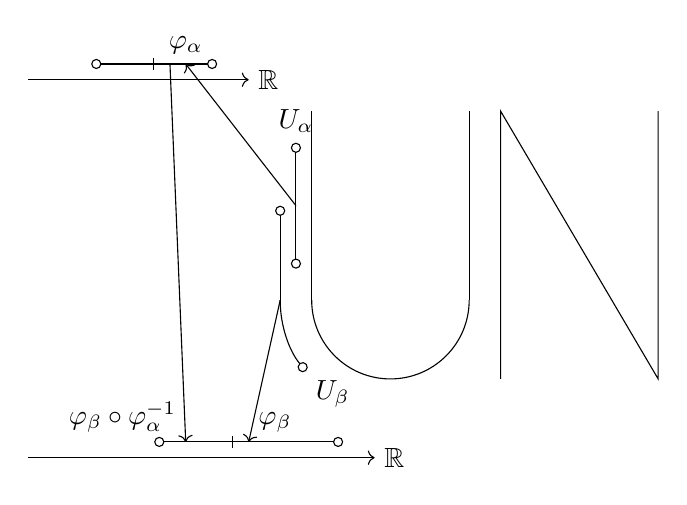
\begin{tikzpicture}[scale=4]
        \draw(0,0.6) -- (0,0);
        \draw(0.5,0.6) -- (0.5,0.0);
        \draw (0,0) arc (180: 360: 0.25); 
        \draw (0.6, -0.25) -- (0.6,0.6) -- (1.1,-0.25) -- (1.1,0.6); 
        \draw[{Circle[open]}-{Circle[open]}]   (-0.05,0.5) node[above] {$U_\alpha$}-- (-0.05, 0.1);
        \draw[{Circle[open]}-] (-0.1,0.3) -- (-0.1,0);
        \draw[-{Circle[open]}] (-0.1,0.0) arc (180:220: 0.35) node[below right] {$U_\beta$};
        \draw[->] (-0.05,0.3) -- (-0.4,0.75) node[above] {$\varphi_\alpha$};
        \draw[->] (-0.9,0.7) --(-0.2,0.7) node[right] {$\mathbb{R}$};
        \draw[{Circle[open]}-{Bar}] (-0.7,0.75) -- (-0.5,0.75); 
        \draw[-{Circle[open]}] (-0.5,0.75) -- (-0.3,0.75);
        \draw[->] (-0.1,0) -- (-0.2,-0.45) node[above right] {$\varphi_\beta$};
        \draw[->] (-0.9,-0.5) -- (0.2, -0.5) node[right] {$\mathbb{R}$};
        \draw[{Circle[open]}-{Bar}] (-0.5, -0.45) -- (-0.25,-0.45);
        \draw[-{Circle[open]}] (-0.25,-0.45) -- (0.1,-0.45);
        \draw[->] (-0.45,0.75) -- (-0.4,-0.45) node[above left] {$\varphi_\beta \circ \varphi_\alpha^{-1}$};
      \end{tikzpicture}
    \end{figure}

    74) Album [2]
    \[
        \Delta C 
    \]

    75) Show [2]
       \[                                            
         A\cos \omega_1 t, \text{ } A \cos \omega_2 t
       \]   

    76) Song [4]
      \begin{figure}[htbp!]
    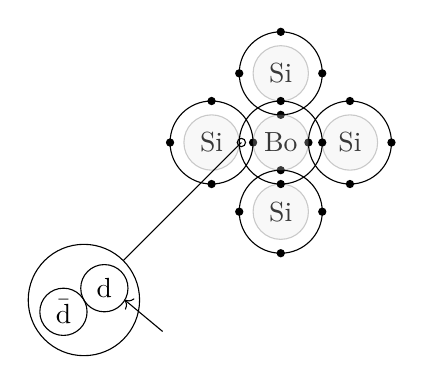
\begin{tikzpicture}[
    baseline=(nucleus.base),
    nucleus options/.style = {draw=black!80,fill=black!10,opacity=.25},
    shell options/.style = {draw=black!100,thin},
    electron options/.style = {black!100},
    silicon/.pic = {
      \node (nucleus) at (0,0) {Si};
      \draw[nucleus options] (nucleus) circle (1em);
      \draw[shell options] (nucleus) circle (1.5em);
      \foreach \angle in {0,90,180,270} {
        \fill[electron options] (nucleus) ++(\angle:1.5em) circle (1.5pt);
      }
    },
     boron/.pic = {
      \node (nucleus) at (0,0) {Bo};
      \draw[nucleus options] (nucleus) circle (1em);
      \draw[shell options] (nucleus) circle (1.5em);
      \foreach \angle in {0,90,270} {
        \fill[electron options] (nucleus) ++(\angle:1.5em) circle (1.5pt);
      }
    },
    ]

    \foreach \angle in {0,90,180,270} {
      %\fill[lightgray,rotate=\angle] (1.7em,0) ellipse (0.2em and .5em);
      \path (1.5,1.5)  ++ (\angle:2.5em) pic {silicon};
    }
      \path (1.5,1.5) pic {boron};
      \draw[-] (-0.5,0) -- (1,1.5);
			\draw (1,1.5) circle (1.5pt);
			\begin{scope}[shift={(-1,-0.5)}]
			\draw (0,0) circle ({0.5*sqrt(2)});
			\draw (30:0.3) circle (0.3) node {d};
			\draw (210:0.3) circle (0.3) node {$\bar{\text{d}}$};
			\draw[<-] ({0.3*cos(30)+0.3*cos(30)},0) -- (1,-0.4); 
			\end{scope}
			%\draw (
      %\node at (4.5,1.5) {$r_s = \frac{2GM}{c^2}$};
      %\node at (7,1.5) {$T_1 = \sum_{i} \sum_{a} t^i_a \hat{a}^a \hat{a}_i$};
    \end{tikzpicture}
   \end{figure}
   
    77) Show [3]
    \begin{figure}[htbp!]
      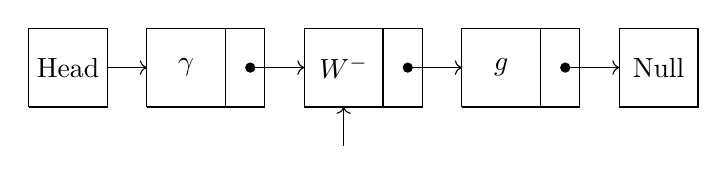
\begin{tikzpicture}
      \foreach \i in {0,2,4} {
        \draw (0+\i,0) --(1+\i,0) -- (1+\i,1) -- (0+\i,1) -- (0+\i,0);
        \draw (1+\i,1) -- (1.5+\i,1) -- (1.5+\i,0) -- (1+\i,0);
        \draw[{Circle}->] (1.25+\i,0.5) -- (2+\i,0.5);
      }
        \draw[->] (-0.5,0.5) -- (0,0.5);
        \node at (-1,0.5) {Head};
        \draw (-1.5,0) -- (-0.5,0) -- (-0.5,1) -- (-1.5,1) -- (-1.5,0);
        \draw (6,0) -- (6,1) -- (7,1) -- (7,0) -- (6,0);
        \node at (6.5,0.5) {Null};
        \node at (0.5,0.5) {$\gamma$};
        \node at (2.5,0.5) {$W^-$};
        \draw[->] (2.5,-0.5) -- (2.5,0);
				\node at (4.5,0.5) {$g$};
      \end{tikzpicture}
    \end{figure}

      78) Song [4]
      \[
      \heartsuit  \in \clubsuit
      \]

      79) Album/Song [3]
      \[
        \text{Ag}\si{\deci\bel}
      \]

      80) Film [3]
      \begin{figure}[htbp!]
      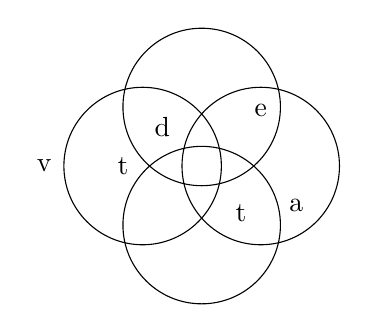
\begin{tikzpicture}
        \foreach \angle in {0,90,180,270} {
        \draw (\angle:0.75cm) circle (1cm);
      };
        \node at (-2,0) {v};
        \node at (-0.5,0.5) {d};
        \node at (0.75,0.7) {e};
        \node at (-1,0) {t};
        \node at (0.5,-0.6) {t};
        \node at (1.2,-0.5) {a};
      \end{tikzpicture}
      \end{figure}
   
    81) Film [3]
      \[
        S = \int L_1 \dd{t}, \text{ } \mathcal{S} = \int L_2 \dd{t},\text{ }\ldots, \text{ } \underbrace{\Superman = \int L_n \dd{t}}_{\text{this}}    
      \]
    82) Book/Film [4]
    \[
      \text{For group element \PHeagle, smallest } m \text{ such that } \text{\PHeagle}^m = E
    \]

    83) Film [3]
    \begin{figure}[htbp!]
      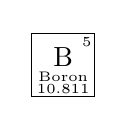
\begin{tikzpicture}
        \draw (0,0) -- (0.8,0) -- (0.8,0.8) -- (0,0.8) -- (0,0);
        \node at (0.4,0.5) {B};
        \node at (0.4, 0.25) {\centering \tiny Boron};
        \node at (0.4, 0.1) {\centering \tiny 10.811};
        \node at (0.7,0.7)  {\tiny 5};
      \end{tikzpicture}
    \end{figure}

    84) Show [3]
    \[
        -\SI{1.8288}{\metre}
    \]

    85) Book/Film [5]
    \[
      \sum_{i=1}^{U_N} (\text{Lucky Incident})_i
    \]

    86) Book/Film [3]
    \[
      \pi^0 \ce{ -> } 2 \gamma
    \]

    87) Film/Song (spelt differently) [1] or [2] 
    \[
        a \times 10^{-3}
    \]

    88) Film (Sophus Lie...) [1]
    \[
      a\mathcal{L}_{N}(S)    
\]

		\[
		\begin{split}
			&[\cdot,\cdot]: \mathfrak{g} \times \mathfrak{g} \to \mathfrak{g}	\\
			&	a[n,s] \\
		\end{split}	
\]

    89) Film [2]
  \[
      \nabla u_8
  \]

  91) Book [1]
  \[
    \begin{split}
      &tx_1 + (1-t)x_2 \text{ where} \\
      &x_1 = \text{March 1} \\
      &x_2 = \text{April 1} \\
      &t = 0.5 \\
    \end{split}
    \]

  92) Film [2]
  \[
      3\orca
  \]

  93) Albums
  \[
  \text{Using } \ce{Pb} \text{ with } \ce{H2}
  \]

  94) Books/Films [5]
  \[
    \begin{split}
      &\symking, \text{ where} \\
      &\{ \Phi | \Phi  \text{ is a set } R \text{ equipped with binary operations } + \text{ and } \cdot \\
      &\text{ (addition and multiplication, respectively) such that }\\
      &R \text{ is abelian under addition, a monoid under multiplication, }\\
      &\text{and multiplication is distributive with respect to addition} \} \in \symking\\
    \end{split}
  \]

  95) Album [3]
  \[
      \frac{h}{\lambda}, \text{ } \lambda \sim \SI{470}{\nano\meter}
  \]

  96) Film [3]
  \[
    \underbrace{e^n} -\underbrace{d} + \underbrace{\text{\fontspec{Symbola.ttf} 👂}} + \underbrace{\male t}
  \]

  97) Album/Songs [3]
    \begin{figure}[htbp!]
      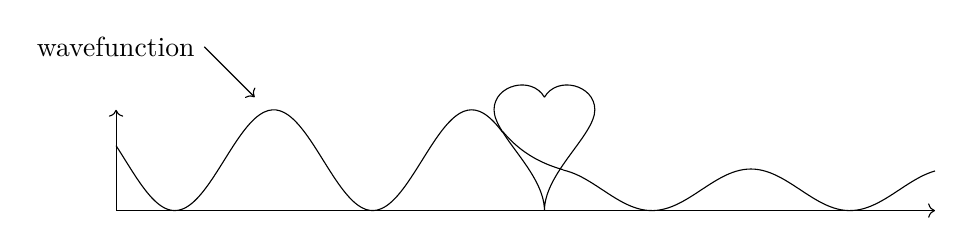
\begin{tikzpicture}[scale=0.16]
      \draw[]  (4,1) ..controls +(120:2cm)
        and +(90:2cm) .. (0,0) .. controls  +(-90:2cm) and +(90:3cm) ..
        (4,-8) .. controls +(90:3cm) and +(-90:2cm) ..(8,0)  .. controls
        +(90:2cm) and  +(60:2cm) .. (4,1);
				\draw[->] (-23,5) node[left] {wavefunction} -- (-19,1);
	      \draw[<->] (-30,0)   -- (-30,-8) -- (35,-8);
        \draw[smooth, samples=100, domain=-30:0.67] plot (\x, {4*sin(deg(0.4*\x)-deg(4))-4});
        \draw[smooth, samples=100, domain=0.67:5.5] plot (\x, {4*exp(-0.3*\x+0.67*0.3)-5.7});
        \draw[smooth, samples=100, domain=5.5:35] plot (\x, {1.65*sin(deg(0.4*\x)-deg(0.3))-6.35});
      \end{tikzpicture}
    \end{figure}

    \begin{tabular}{ccc}
      $-\frac{\hbar^2}{2m}\psi''(x) = E\psi(x)$ & $-\frac{\hbar^2}{2m} \psi''(x) = (E - \heartsuit)\psi(x)$ & $-\frac{\hbar^2}{2m}\psi''(x) = E \psi(x)$ \\
      $x < 0$ & $0 \leq x \leq L$, $\heartsuit > E$ & $x > L$ \\
    \end{tabular}
  

    98) Film [6]
    \begin{figure}[htbp!]
      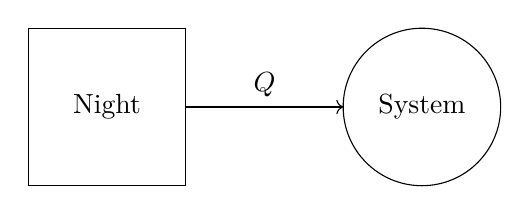
\begin{tikzpicture}
        \draw[-] (0,0) -- (2,0) -- (2,2) -- (0,2) -- (0,0);
        \node at (1,1) {\text{Night}};
        \draw[->] (2,1) -- (3,1) node[above] {$Q$} -- (4,1);
        \draw (5,1) circle[radius = 1];
        \node at (5,1) {\text{System}};
      \end{tikzpicture}
    \end{figure}

    99) Song [1]
    \[
      \text{A bad name for entropy}
    \]

    100) Song [4] and Song [2]
    \begin{figure}[htbp!]
	    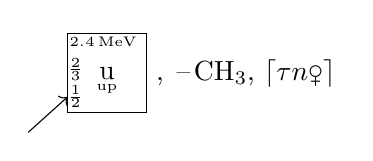
\begin{tikzpicture}
        	\draw (0,0) -- (1,0) -- (1,1) -- (0,1) -- (0,0);
		\node at (0.45,0.9) {\tiny $\SI{2.4}{\mega \electronvolt}$};
		\node at (0.1,0.55) {\tiny $\tfrac{2}{3}$};
		\node at (0.1,0.2) {\tiny $\tfrac{1}{2}$};
	       	\node at (0.5,0.5) {u};
	        \node at (0.5, 0.3) {\centering \tiny up};
		\node[right] at (1,0.5) {, \ce{-CH3}, $\left \lceil \tau n \female \right \rceil $}; 
   		\draw[->] (-0.5,-0.25) -- (0,0.2);	
      \end{tikzpicture}
      \end{figure}

    101) Film [1]
    \[
      \left| \dv{\vec{r}}{ t} \right|
    \]

    102) Film [3]
    \begin{figure}[htbp!]
      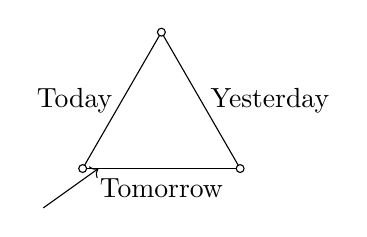
\begin{tikzpicture}
        \draw[-] (0,0) -- (60:1) node[left] {Today} -- (60:2);
        \draw[-] (60:2) -- +(300:1) node[right] {Yesterday} -- (2,0);
        \draw[-] (0,0) -- (1,0) node[below] {Tomorrow} -- (2,0);
        \draw[fill=white] (0,0) circle[radius=0.05];
        \draw[fill=white] (60:2) circle[radius=0.05];
        \draw[fill=white]  (2,0) circle[radius=0.05];
        \draw[->] (-0.5,-0.5) -- (0.2,0);
      \end{tikzpicture}
    \end{figure}

    103) Game [2]
    \[
        \begin{split}
          &R_{\mu \nu} - \tfrac12 Rg_{\mu \nu} + \Lambda g_{\mu \nu} = \frac{8 \pi G}{c^4 }T_{\mu \nu} \\
          &\text{The RHS's impact on the LHS}
        \end{split}
    \]

    104) Song [2]
    \[
      \forall n \in \mathbb{N}:  \dv[n]{\text{Thief}(x)}{x} \text{ exists}
    \]
      
    105) Film [2]
    \[
        \text{Fe male}
    \]

    106) Show [3]
    \begin{figure}[htbp!]
      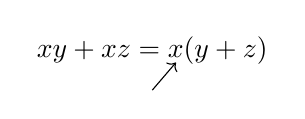
\begin{tikzpicture}
        \node at (0,0) {$xy + xz = x(y+z)$};
        \draw[->] (0,-0.5) -- (0.3, -0.15);
      \end{tikzpicture}
    \end{figure}
    
    107) Film [2]
    \begin{figure}[htbp!]
      \begin{tikzpicture} 
        \draw[->] node[below left] {e$^+$} (0,0) -- node[above]{$\vec{F}$} (1,0.5) ;
        \draw[<-]   (2,1) -- node[above] {$\vec{F}$} (3,1.5)  node[above right] {e$^-$};
      \end{tikzpicture}
    \end{figure}

    108) Film [2]
    \[
      \text{LA}^{+ \text{tial}}_{-\text{\{ce interval\}}}
    \]

    109) Album [1]
    \[
      x^2
    \]
    
    110) Film [2]
    \[
      \text{term} \in (8  \lor 2)
    \]

    111) Film [4]
    \[
        \begin{pmatrix}
          -1 & 0 & 0 \\
          0 & -1 & 0 \\
          0 & 0  & 1 \\
        \end{pmatrix}
    		\begin{pmatrix} 
					\text{\symking}_x  \\    
   				\text{\symking}_y  \\
					\text{\symking}_z
				\end{pmatrix}
\]

    112) Film [2]
    \[
      \texttt{investigator = !(6<=4)}
    \]

    113) Film [2]
    \[
        \frac{1}{N} \sum_{i=1}^{N}\female_i
\]

    114) Song [4]
    \[
      x^\heartsuit
    \]

    115) Film/Book [4]
    \[
      (\text{Relative to you: } \vec{r}=0 ) \to t = \infty
    \]

    116) Song (also Album/Film with different name) [1]
    \[
        \underbrace{\heartsuit -} x   
    \]

    117) Film [2]
    \begin{figure}[htbp!]
      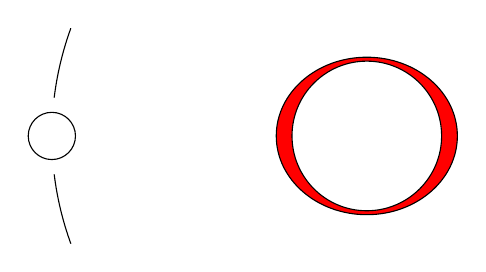
\begin{tikzpicture}[rotate=180]
        \draw[fill=red] (0,0) circle (1.15 and 1);
        \draw[fill = white] (0,0) circle (0.95);
        \draw (4,0) circle (0.3);
				\draw ({4*cos(7)},{4*sin(7)}) arc (7:20:4);    
	    	\draw ({4*cos(-7)},{4*sin(-7)}) arc (-7:-20:4);
			\end{tikzpicture}
    \end{figure}

    118) Film [2]
    \[
      a_\text{Ghost} = e^{\frac{\mu_\text{Ghost} - \mu_\text{Ghost}^\ominus}{RT}}
    \]

    119) Song [2]
    \[
    \begin{split}
      &\text{Teenager}_0 + h f_1 \to \text{Teenager}_1 \\
      &\text{Teenager}_1 \to \text{Teenager}_2 + h f_2 \\
      &f_1 > f_2 \\
    \end{split}
    \]

    120) Song [4]
    \[
      \vec{r} \times \vec{F}, \quad \underbrace{\sum_i m_i r_i^2}_{\text{this}}, \quad  q \vec{d}, \quad  \vec{m} \times \vec{B} 
    \]

    121) Film [2]
    
      Point mass with $v>0$ and $a<0$
    

    122) Film [1]
    \begin{figure}[htbp!]
      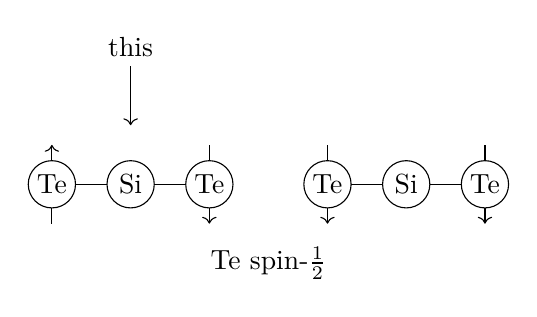
\begin{tikzpicture}
			\draw[->] (-0.75,1.5) node[above] {this} -- (-0.75,0.75);
			\begin{scope}[shift={(-1.75,0)}]
        \draw (0,0) circle (0.3) node {Te};
        \draw (1,0) circle (0.3) node {Si};
        \draw (2,0) circle (0.3) node {Te};
        \draw (0.3, 0) -- (0.7,0);
        \draw (1.3, 0) -- (1.7,0);
        \draw[->] (0,0.3) -- (0,0.5);
        \draw (0,-0.3) -- (0,-0.5);
        \draw (2,0.3) -- (2,0.5);
        \draw[->] (2,-0.3) -- (2,-0.5);
			\end{scope}
			\begin{scope}[shift={(1.75,0)}]
        \draw (0,0) circle (0.3) node {Te};
        \draw (1,0) circle (0.3) node {Si};
        \draw (2,0) circle (0.3) node {Te};
        \draw (0.3, 0) -- (0.7,0);
        \draw (1.3, 0) -- (1.7,0);
        \draw[] (0,0.3) -- (0,0.5);
        \draw[->] (0,-0.3) -- (0,-0.5);
        \draw (2,0.3) -- (2,0.5);
        \draw[->] (2,-0.3) -- (2,-0.5);
			\end{scope}


        \node at (1,-1) {Te spin-$\frac12$};
      \end{tikzpicture}
    \end{figure}

    123) Film [2]
    \begin{figure}[htbp!]
      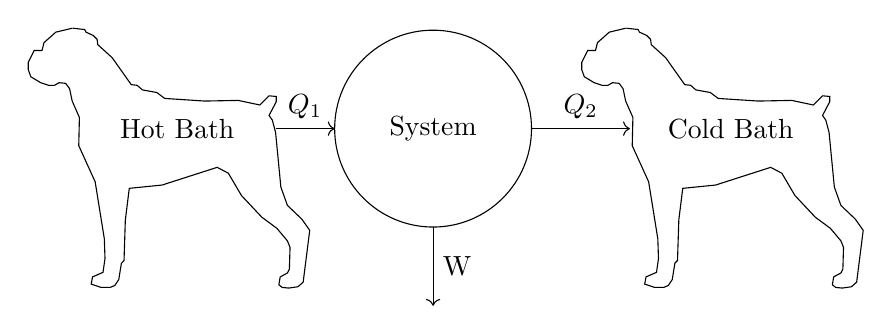
\begin{tikzpicture}[scale=0.25]
               \draw    plot [smooth, tension=0] coordinates { (3.666667,15.1) (2.833333,14.9) (2.233333,14.36667) (2.133333,13.96667) (1.733333,13.96667) (1.433333,13.36667) (1.433333,13) (1.566667,12.63333) (2.066667,12.33333) (2.466667,12.2) (2.766667,12.2) (3,12.33333) (3.333333,12.3) (3.533333,12.03333) (3.666667,11.4) (4.033333,10.56667) (4,9.133333) (4.833333,7.3) (5.3,4.4) (5.333333,3.4) (5.233333,2.7) (4.7,2.466667) (4.633333,2.1) (5.133333,1.933333) (5.6,1.933333) (5.833333,2.033333) (6.033333,2.333333) (6.166667,3.166667) (6.3,3.3) (6.366667,5.366667) (6.566667,6.966667) (8.233334,7.133333) (11.03333,8.033334) (11.6,7.733333) (12.26667,6.6) (13.3,5.5) (14.06667,4.933333) (14.6,4.3) (14.73333,3.966667) (14.7,2.866667) (14.6,2.666667) (14.23333,2.466667) (14.16667,2.066667) (14.33333,1.933333) (14.66667,1.9) (15.13333,1.966667) (15.4,2.2) (15.73333,4.833333) (15.33333,5.4) (14.6,6.1) (14.26667,7.033333) (14,9.8) (13.83333,10.43333) (13.66667,10.66667) (14.03333,11.36667) (14.03333,11.63333) (13.66667,11.66667) (13.2,11.2) (12.1,11.43333) (10.4,11.4) (8.366667,11.53333) (7.966667,11.83333) (7.233333,11.96667) (6.966667,12.2) (6.666667,12.23333) (5.7,13.6) (4.966667,14.26667) (4.933333,14.53333) (4.733333,14.73333) (4.366667,14.9) (4.3,15.03333) (3.7,15.1) };
        \begin{scope}[xshift = 800] 
           \draw    plot [smooth, tension=0] coordinates { (3.666667,15.1) (2.833333,14.9) (2.233333,14.36667) (2.133333,13.96667) (1.733333,13.96667) (1.433333,13.36667) (1.433333,13) (1.566667,12.63333) (2.066667,12.33333) (2.466667,12.2) (2.766667,12.2) (3,12.33333) (3.333333,12.3) (3.533333,12.03333) (3.666667,11.4) (4.033333,10.56667) (4,9.133333) (4.833333,7.3) (5.3,4.4) (5.333333,3.4) (5.233333,2.7) (4.7,2.466667) (4.633333,2.1) (5.133333,1.933333) (5.6,1.933333) (5.833333,2.033333) (6.033333,2.333333) (6.166667,3.166667) (6.3,3.3) (6.366667,5.366667) (6.566667,6.966667) (8.233334,7.133333) (11.03333,8.033334) (11.6,7.733333) (12.26667,6.6) (13.3,5.5) (14.06667,4.933333) (14.6,4.3) (14.73333,3.966667) (14.7,2.866667) (14.6,2.666667) (14.23333,2.466667) (14.16667,2.066667) (14.33333,1.933333) (14.66667,1.9) (15.13333,1.966667) (15.4,2.2) (15.73333,4.833333) (15.33333,5.4) (14.6,6.1) (14.26667,7.033333) (14,9.8) (13.83333,10.43333) (13.66667,10.66667) (14.03333,11.36667) (14.03333,11.63333) (13.66667,11.66667) (13.2,11.2) (12.1,11.43333) (10.4,11.4) (8.366667,11.53333) (7.966667,11.83333) (7.233333,11.96667) (6.966667,12.2) (6.666667,12.23333) (5.7,13.6) (4.966667,14.26667) (4.933333,14.53333) (4.733333,14.73333) (4.366667,14.9) (4.3,15.03333) (3.7,15.1) };
        \node at (9,10) {Cold Bath};
        \end{scope}     
        \node at (9,10) {Hot Bath};
        \draw[->] (14,10) -- (15.5,10) node[above] {$Q_1$} -- (17,10);
        \draw[->] (27,10) -- (29.5,10) node[above] {$Q_2$} -- (32,10);
        \draw (22,10) circle (5) node {System};
        \draw[->] (22,5) -- (22,3) node[right] {W} -- (22,1);
      \end{tikzpicture}
    \end{figure}

    124) Film [3]
    \[
      \begin{split}
        &\texttt{cd} \\
        &\texttt{pwd} \\
        &\texttt{ls} \\
        &\texttt{cat} \\
        &\texttt{cp} \\
        &\texttt{mv} \\
        &\texttt{mkdir} \\
        &\texttt{rmdir} \\
        &\texttt{rm} \\
        &\texttt{touch} \\
      \end{split}
      \]

    125) Song [4]
    \[
        \frac{w+h+e+r+e}{\prideflag}
    \]

    126) Song [5]
    \begin{figure}[htbp!]
      \begin{tikzpicture}
        \draw (0,0) circle (0.8);
        \draw (5,0) circle (0.25);
        \draw (5 + 0.968246,0.25) arc (14.47:360-14.47:1);
        \node at (6,-0.05) {\heartsuit};
        \draw (4.98097349046,0.43577871373) arc (5:20:5); 
        \draw (4.69846310393, -1.71010071663) arc (340:355:5); 
      \end{tikzpicture}
    \end{figure}

    127) Album/Songs (Very similar names) [3] or [2]
    
    \begin{figure}[htbp!]
      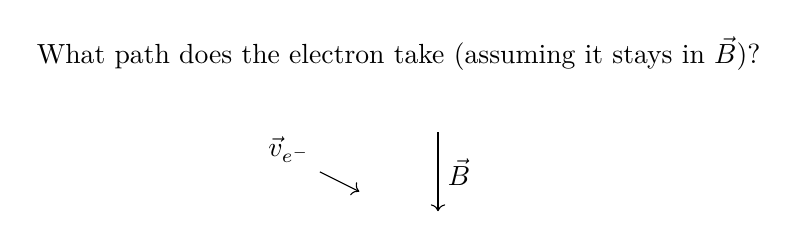
\begin{tikzpicture}
        \node at (1,1.5) {What path does the electron take (assuming it stays in $\vec{B}$)?}; 
        \draw[->] node[above left] {$\vec{v}_{e^-}$} (0,0) -- (0.5,-0.25); 
        \draw[->]   (1.5,0.5) -- (1.5,0) node[right] {$\vec{B}$} --(1.5,-0.5);
      \end{tikzpicture}
    \end{figure}

    128) Song [2]
     \begin{figure}[htbp!]
      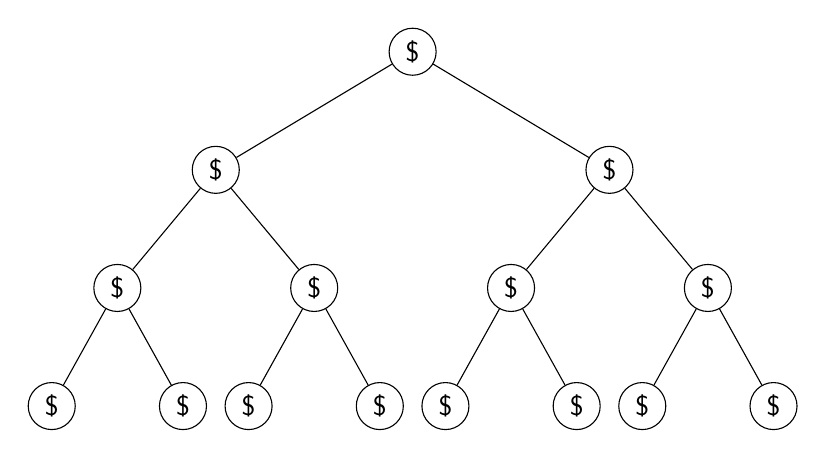
\begin{tikzpicture}[level/.style={sibling distance = 5cm/#1,
  level distance = 1.5cm}] 
\node [arn_n] {\$}
    child{ node [arn_n] {\$} 
            child{ node [arn_n] {\$} 
              child{ node [arn_n] {\$}} 
							child{ node [arn_n] {\$}}
            }
            child{ node [arn_n] {\$}
							child{ node [arn_n] {\$}}
							child{ node [arn_n] {\$}}
            }                            
    }
    child{ node [arn_n] {\$}
            child{ node [arn_n] {\$} 
							child{ node [arn_n] {\$}}
							child{ node [arn_n] {\$}}
            }
            child{ node [arn_n] {\$}
							child{ node [arn_n] {\$}}
							child{ node [arn_n] {\$}}
            }
		}
; 
\end{tikzpicture}
    \end{figure} 

    129) Album/Song [1]
    \[
      \int f(x) \dd{x}, \text{  } \int g(x) \dd{x},\text{  } \underbrace{\int h(x) \dd{x}}_{\text{dis}}
    \]

    130) Show [1]
     \[
       \begin{split}
         &\chemfig{(=[2]Er)-[:-30]Ng} \\
         &\text{Ng = He, Ne, Ar, Kr, Xe, Rn}\\
        \end{split}
    \]

    131) Show [2]
    \begin{figure}[htbp!]
      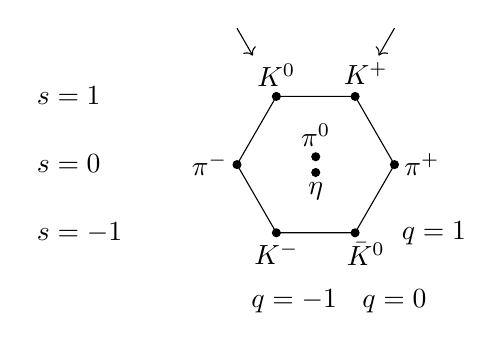
\begin{tikzpicture}
        \draw[->] (60:2) -- (60:1.6);
        \draw[->] (120:2) -- (120:1.6);
        \draw[fill=black] (0:1) circle [radius=0.05] node[right] {$\pi^+$};
        \draw[fill=black] (60:1) circle [radius=0.05] node[above] {$\phantom{-}K^+$};
          \draw[fill=black] (120:1) circle [radius=0.05] node[above] {$K^0$};
          \draw[fill=black] (180:1) circle [radius=0.05] node[left] {$\pi^-$};
          \draw[fill=black] (240:1) circle [radius=0.05] node[below] {$K^-$};
          \draw[fill=black] (300:1) circle [radius=0.05] node[below] {$\phantom{-}\bar{K}^0$};
          \draw[fill=black] (0,0.1) circle [radius=0.05] node[above] {$\pi^0$};
          \draw[fill=black] (0,-0.1) circle [radius=0.05] node[below] {$\eta$};
          \draw[-] (0:1) -- (60:1) -- (120:1) -- (180:1) -- (240:1) -- (300:1) -- (360:1);
          \node at (-3,0) {$s=0\phantom{-}$};
          \node at (-3,0.86602540378) {$s=1\phantom{-}$};
          \node at (-3,-0.86602540378) {$s=-1$};
          \node at (1+0.5,-0.86602540378) {$q=1$};
          \node at (1, -2*0.86602540378) {$q=0$};
          \node at (0,-2*0.86602540378) {$q=-1\phantom{--}$};
      \end{tikzpicture}
      \end{figure}
    
    
    132) Game [2]
      \begin{figure}[htbp!]
        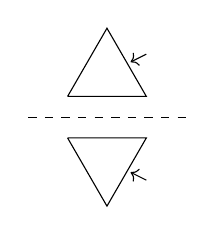
\begin{tikzpicture}

          \begin{scope}[yshift=7.5]
          \draw[-] (0,0) --  (1,0) -- + (120:1) --  (0,0);
          \end{scope}
          \begin{scope}[yshift=-7.5]
          \draw[-] (0,0) --  (1,0) -- + (240:1) --  (0,0);
          \end{scope}
          \draw[dashed] (-0.5,0) --(1.5,0);
          \draw[->] (1,0.8) --(0.8,0.7);
          \draw[->] (1,-0.8) --(0.8,-0.7);
        \end{tikzpicture}
      \end{figure}

    133) Film [5]
    \[
      \min_{x}|\text{It}(x) - \text{Good}(x)|
    \]

    134) Film [2]
    \[
      2 \times \text{LossProtection}
    \]

    135) Film [3]
    \begin{figure}[htbp!]
      \centering
      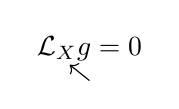
\begin{tikzpicture}   
        \node at (0,0) {$\mathcal{L}_{X} g = 0$};
        \draw[->] (0,-0.4) -- (-0.25,-0.2);
      \end{tikzpicture}
    \end{figure}

    136) Book [1]
    \[
      9 \leq \female \leq 14
    \]

    137) Song [4]
    \[
      \boldsymbol{1}.034\boldsymbol{1}28\boldsymbol{1}73\SI{92}{\second}= \int_{0}^{\infty} t \lambda e^{-t/\lambda} \dd{t}
    \] 

    138) Song [2]
    \begin{figure}[htbp!]
      \centering
      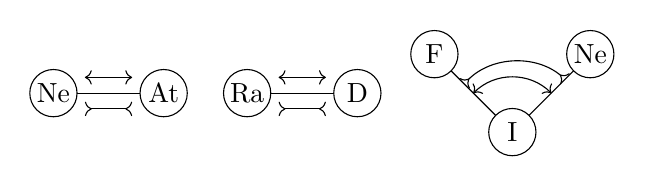
\begin{tikzpicture}
        \draw(-0.7,0) circle (0.3) node {Ne};
        \draw(0.7,0) circle(0.3) node{At};
        \draw[-] (-0.4,0) -- (0.4,0);
        \draw[<->] (-0.3,0.2) -- (0.3,0.2);
        \draw[>-<] (-0.3,-0.2) -- (0.3,-0.2);
      \begin{scope}[xshift = 70]
        \draw(-0.7,0) circle (0.3) node {Ra};
        \draw(0.7,0) circle(0.3) node{D};
        \draw[-] (-0.4,0) -- (0.4,0);
        \draw[<->] (-0.3,0.2) -- (0.3,0.2);
        \draw[>-<] (-0.3,-0.2) -- (0.3,-0.2);
      \end{scope}
      \begin{scope}[xshift = 160, rotate=45]
        \draw(-0.7,1.4) circle (0.3) node{F};
        \draw(-0.7,0) circle (0.3) node {I};
        \draw(0.7,0) circle(0.3) node{Ne};
        \draw[-] (-0.4,0) -- (0.4,0);
        \draw[-] (-0.7,0.3) -- (-0.7,1.1); 
        \draw[<->] (0,0) arc (0:90:0.7);
        \draw[>-<] (0.25,0) arc (5:90:0.95);
      \end{scope} \end{tikzpicture}
    \end{figure}

      139) Film [6]
      \[
        \text{Age}(t) = 80 - t
      \]

      139) Song [1]
      
      140) Series [1] 
      \[
        f \text{ where } f(x) = x + \text{Black}
      \]

      141) Song [5]
      \[
\schemestart
\chemfig{US}
      \arrow{->[LuV]} 
\chemfig{U}
\chemfig{+}
\chemfig{S}
\schemestop
\]

	142) Game [2]
	\[
	L_\text{sol} = \sigma AT^4, \text{ } T=0
	\]
	
	143) Film [4]
	\begin{figure}[htbp!]
	\centering
      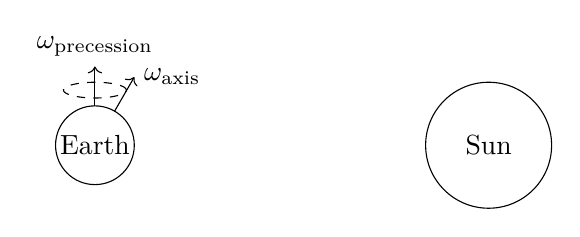
\begin{tikzpicture}
        \draw (0,0) circle (0.5) node {Earth};
        \draw (5,0) circle (0.8) node {Sun};
        \draw[->] (60:0.5) -- (60:1) node[right] {$\omega_{\text{axis}}$};
        \draw[->] (0,0.5) -- (0,1) node[above] {$\omega_{\text{precession}}$};
        \draw[dashed] (0,0.7) circle (0.4 and 0.1);
      \end{tikzpicture}
    \end{figure}
    \[
    	\omega_{\text{precession}}(t) = \begin{cases}
    	\frac{2\pi}{T_\text{orbit}}, & 0 \leq t \leq T \\
    	0, & t \geq T \\
    	\end{cases}
    \]
    \[
    \text{where }T> T_\text{orbit}  \text{ and it is part of the answer.}
    \]
    
    144) Film [2]
    \[
    |\{ x| x \in \text{house}\}| =1 
    \]
    
    145) Film [4] 
    
		\begin{figure}[htbp!]
		\centering
      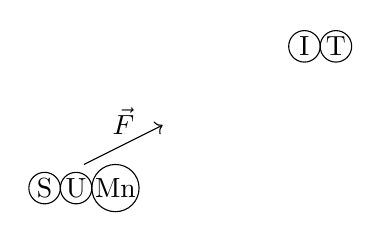
\begin{tikzpicture} 
        \draw[->] (0,0) -- node[above]{$\vec{F}$} (1,0.5) ;
       	\draw (-0.5,-0.3) circle (0.2)  node{S};
       	\draw (-0.1,-0.3) circle (0.2) node{U};
    	\draw (0.4,-0.3) circle (0.3) node{Mn};
        \draw  (2.8,1.5) circle (0.2)  node {I};
        \draw (3.2,1.5) circle (0.2) node{T};
      \end{tikzpicture}
    \end{figure}
    \[
    F = \alpha T_\text{IT} \text{ where }\alpha \text{ is a constant.}
	\]    
    
    146) Film [4]
    {\setboardfontsize{7pt}

    \[
    	m_{ \text{\BlackKnightOnWhite}} a = F - m_ \text{\BlackKnightOnWhite} g
    \]
    \[
    	F > m_ \text{\BlackKnightOnWhite} g
    \]
    }
    
    147) Song [5]
    \[
    \texttt{while(Gibson.numTears()>0)\{\newline
    \ldots
    \}}
    \]
    
    148) Book/Song  [5]
    \[
    \texttt{for(person i : PeopleWhoWillDie)\{\ldots\}}
    \]
    
	149) Song [6]
	\[
	\texttt{while(!Me.HadEnough())\{\ldots\}}
	\]
	
	150) Song [3]
	\[
    \begin{split}
      \text{c}\bar{\text{d}}&\ce{ -> }\bar{\text{u}}\text{s} +\text{u}\bar{\text{d}} + \bar{\text{u}}\text{d} \\
      \text{c}\bar{\text{u}}&\ce{ -> } \bar{\text{u}}\text{s} +\text{u}\bar{\text{d}} \\
      \text{c}\bar{\text{s}}&\ce{ -> } \text{u}\bar{\text{s}} + \bar{\text{u}}\text{s} + \text{u}\bar{\text{d}}
    \end{split}
    \]
	
	151) Song [3]
	\begin{figure}[htbp!]
		\centering
		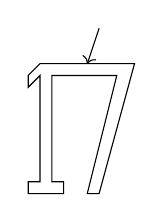
\begin{tikzpicture}[scale=1.5]
		\draw[-] (0,0) --(-0.1,0) --(-0.1,0.1) --(0,0.1) -- (0,1)--(-0.1,0.9)--(-0.1,1) --(0,1.1) --(0.8,1.1) -- ((0.5,0) -- (0.4,0) -- (0.65,1) -- (0.1,1) -- (0.1,0.1) -- (0.2,0.1) -- (0.2,0) --(0,0);
		\draw[->] (0.5,1.4) -- (0.4,1.1);
		\end{tikzpicture}	
	\end{figure}
	
	152) Film [1]
	\[
	\ce{Se7Ne}
	\]
	
	153) Film [2]
	\[
	e^{3.2i} + 1 = 0
	\]
      
      
     154) Album [2]
     
     \[
      \text{pleasure}_1 \text{ and pleasure}_2 \text{ before }
      \]
      \[ f(\text{pleasure}_1,\text{pleasure}_2) = 0 \text{ is solved for pleasure}_1  \text { and pleasure}_2 
     \]
     
     155) Series [1]
     \[
    \sqrt{s}
     \]
     
     
     
     
   
   
   \end{document}
